\renewcommand{\theequation}{\theenumi}
\begin{enumerate}[label=\thesection.\arabic*.,ref=\thesection.\theenumi]
\numberwithin{equation}{enumi}

\item $aigiri.txt$ contains a stothram in Telugu. The stothram is split into two files $aigiri\_test1.txt$ and $aigiri\_test2.txt$. The three files are read and each telugu character in the file is converted to its unicode value and is written onto $unicode.txt$, $unicode\_test1.txt$ and $unicode\_test2.txt$ respectively.
\begin{lstlisting}[language=Python]
def read(file_name):
  sloka = open(file_name, 'r')
  sloka_txt = sloka.read()
  sloka.close()
  return sloka_txt
\end{lstlisting}

\begin{lstlisting}[language=Python]
def split_to_words(txt, out_file_name):
  words = txt.split()
  uni_file = open(out_file_name, 'w')

  for i in words:
      if(i !='|' and i !='||' and not(i.isdigit())):
          for j in i:
              uni_file.write('U+' + hex(ord(j)).replace('x', ''))
              uni_file.write('  ')

  uni_file.close()
  
split_to_words(read('aigiri_test1.txt'), 'unicode_test1.txt')
split_to_words(read('aigiri_test2.txt'), 'unicode_test2.txt')
split_to_words(read('aigiri.txt'), 'unicode.txt')
\end{lstlisting}

\item $unicode.txt,\  unicode\_test1.txt$ and $unicode\_test2.txt$ are read and are split into a list of individual unicode values with the help of the function $read\_and\_split$. $uni\_chars\_list$ is a list which contains the list of unicode values from $unicode\_test1.txt$ and $unicode\_test2.txt$.
\begin{lstlisting}[language=Python]
uni_chars_list = []
aigiri_chars = read_and_split('unicode.txt')
uni_chars_list.append(read_and_split('unicode_test1.txt'))
uni_chars_list.append(read_and_split('unicode_test2.txt'))
\end{lstlisting}

\item A for loop runs through the list $uni\_chars\_list$. In the first iteration the variable $uni\_chars$ is the list of all the unicode values from the file $unicode\_test1.txt$. Each individual unicode value from the file is taken and its periodicity is found through the function $to\_cal\_periodicity$.
All the unicode values whose periodicity is found is appended to the list $periodicity\_found$. A dictonary called $periodicity$ is created and a key with the name of the unicode value whose periodicity has to been found is added to the dictonary and its value is initialized to an empty list.  
\begin{lstlisting}[language=Python]
for file_no, uni_chars in enumerate(uni_chars_list):
  global periodicity_found 
  global periodicity 
  global processed_periodic_dict 
  global test_results

  if file_no != 0:
    periodicity_found = []
    periodicity = {}
    processed_periodic_dict = {}

  for i, char in enumerate(uni_chars):
    if char in periodicity_found:
      pass
    else:
      periodicity_found.append(char)
      periodicity[char] = []
      to_cal_periodicity(char, i, file_no)
    
  print(periodicity)
  to_process_dict(periodicity)
  print(processed_periodic_dict)
  plot_bar(processed_periodic_dict)
  test_results.append(processed_periodic_dict)
\end{lstlisting}

\item The function $to\_cal\_periodicity$ calculates the periodicity of an unicode value which is passed as an argument. The function also takes in the index of the unicode value and the file number. The function scans all the unicode values in the file from the index and calculates the number of unicode values in between two consequitive occurences of the unicode value passed as an argument. This count is appended to the empty list declared using the previous code.
\begin{lstlisting}[language=Python]
def to_cal_periodicity(char, index, file_no):
    count = 0
    temp = uni_chars_list[file_no][index+1:]
    for j in temp:
        if j == char:
            periodicity[char].append(count)
            count = 0
        else:
            count = count + 1
\end{lstlisting}

\item After excuting the previous function the dictonary $periodicity$ contains all the unique unicode value as its key and each key has a corresponding periodicity list. The function 
$to\_process\_dict$ takes the dictonary $periodicity$ as its argument. It converts all the keys which are presently unicode values to telugu characters and finds the average of the elements in the corresponding list and normalizes the value with the total number of unicode values in the stothram.  
\begin{lstlisting}[language=Python]
def to_process_dict(periodicity_dict):
    dict_keys = periodicity_dict.keys()
    
    for key in dict_keys:
        if len(periodicity_dict[key]) == 0:
            average = 0
        else:
            average = sum(periodicity_dict[key])/len(periodicity_dict[key])
        key = key.replace('U+', '')
        key = key[:1] + 'x' + key[1:]
        processed_periodic_dict[chr(int(key, 16))] = average/len(aigiri_chars)
\end{lstlisting}

\item The function $plot\_bar$ plots the key value pairs of the dictonary $processed\_periodic\_dict$.
\begin{lstlisting}[language=Python]
def plot_bar(periodicity_dict):
    values = list(periodicity_dict.values())
    keys = [ hex(ord(i)).replace('x', '') for i in list(periodicity_dict.keys()) ]

    fig = plt.figure()
    ax = fig.add_axes([0, 0, 5, 5])
    ax.bar(keys, values)
    plt.show()
\end{lstlisting}

\item The same process is repeated for the list of unicode values in the file $unicode\_test2.txt$. The final $processed\_periodic\_dict$ obtained after iterating through each file is appended to the variable $test\_results$.

\item The variable $test\_results$ is a list which contians the processed dictonary of both the files. The common keys between these two dictonaries is found and is appended to the list $common\_keys$ 
\begin{lstlisting}[language=Python]
common_keys = []
test1_result, test2_result = test_results

for i in  list(test1_result.keys()):
  if i in list(test2_result.keys()):
    common_keys.append(i)
\end{lstlisting}

\item Two new dictonaries are $key\_value\_1$ and $key\_value\_2$ are created. $key\_value\_1$ contains keys form the list $common\_keys$ and the corresponding value which is obtained from the processed dictonary of file 1.  $key\_value\_2$ contains keys form the list $common\_keys$ and the corresponding value which is obtained from the processed dictonary of file 2. The key value pairs of both these dictonaries are plotted to see if the pattern found from $aigiri\_test1.txt$ is also present in $aigiri\_test2.txt$.
\begin{lstlisting}[language=Python]
x_pos = np.linspace(0, 9, 41)
barWidth = 0.05
fig = plt.subplots(figsize =(20, 20)) 
common_keys = [ ord(i) for i in common_keys ]

plt.bar(x_pos, list(key_value_1.values()), color ='r', width = barWidth, 
		edgecolor ='grey', label ='aigiri_test1') 
plt.bar(x_pos + barWidth, list(key_value_2.values()), color ='g', width = barWidth, 
		edgecolor ='grey', label ='aigiri_test2') 

plt.xticks(x_pos, common_keys)
plt.legend()
plt.savefig('normalized.png')
plt.savefig('normalized.eps')
plt.show() 
\end{lstlisting}

\newpage
\item The result obtained is \textbf{\ref{fig:bar}}. It can be observed that the periodicity of most characters obtained from $aigiri\_test1.txt$ follows the same pattern in the remaining verses of the stothram. 
\begin{figure}[!t]
\centering
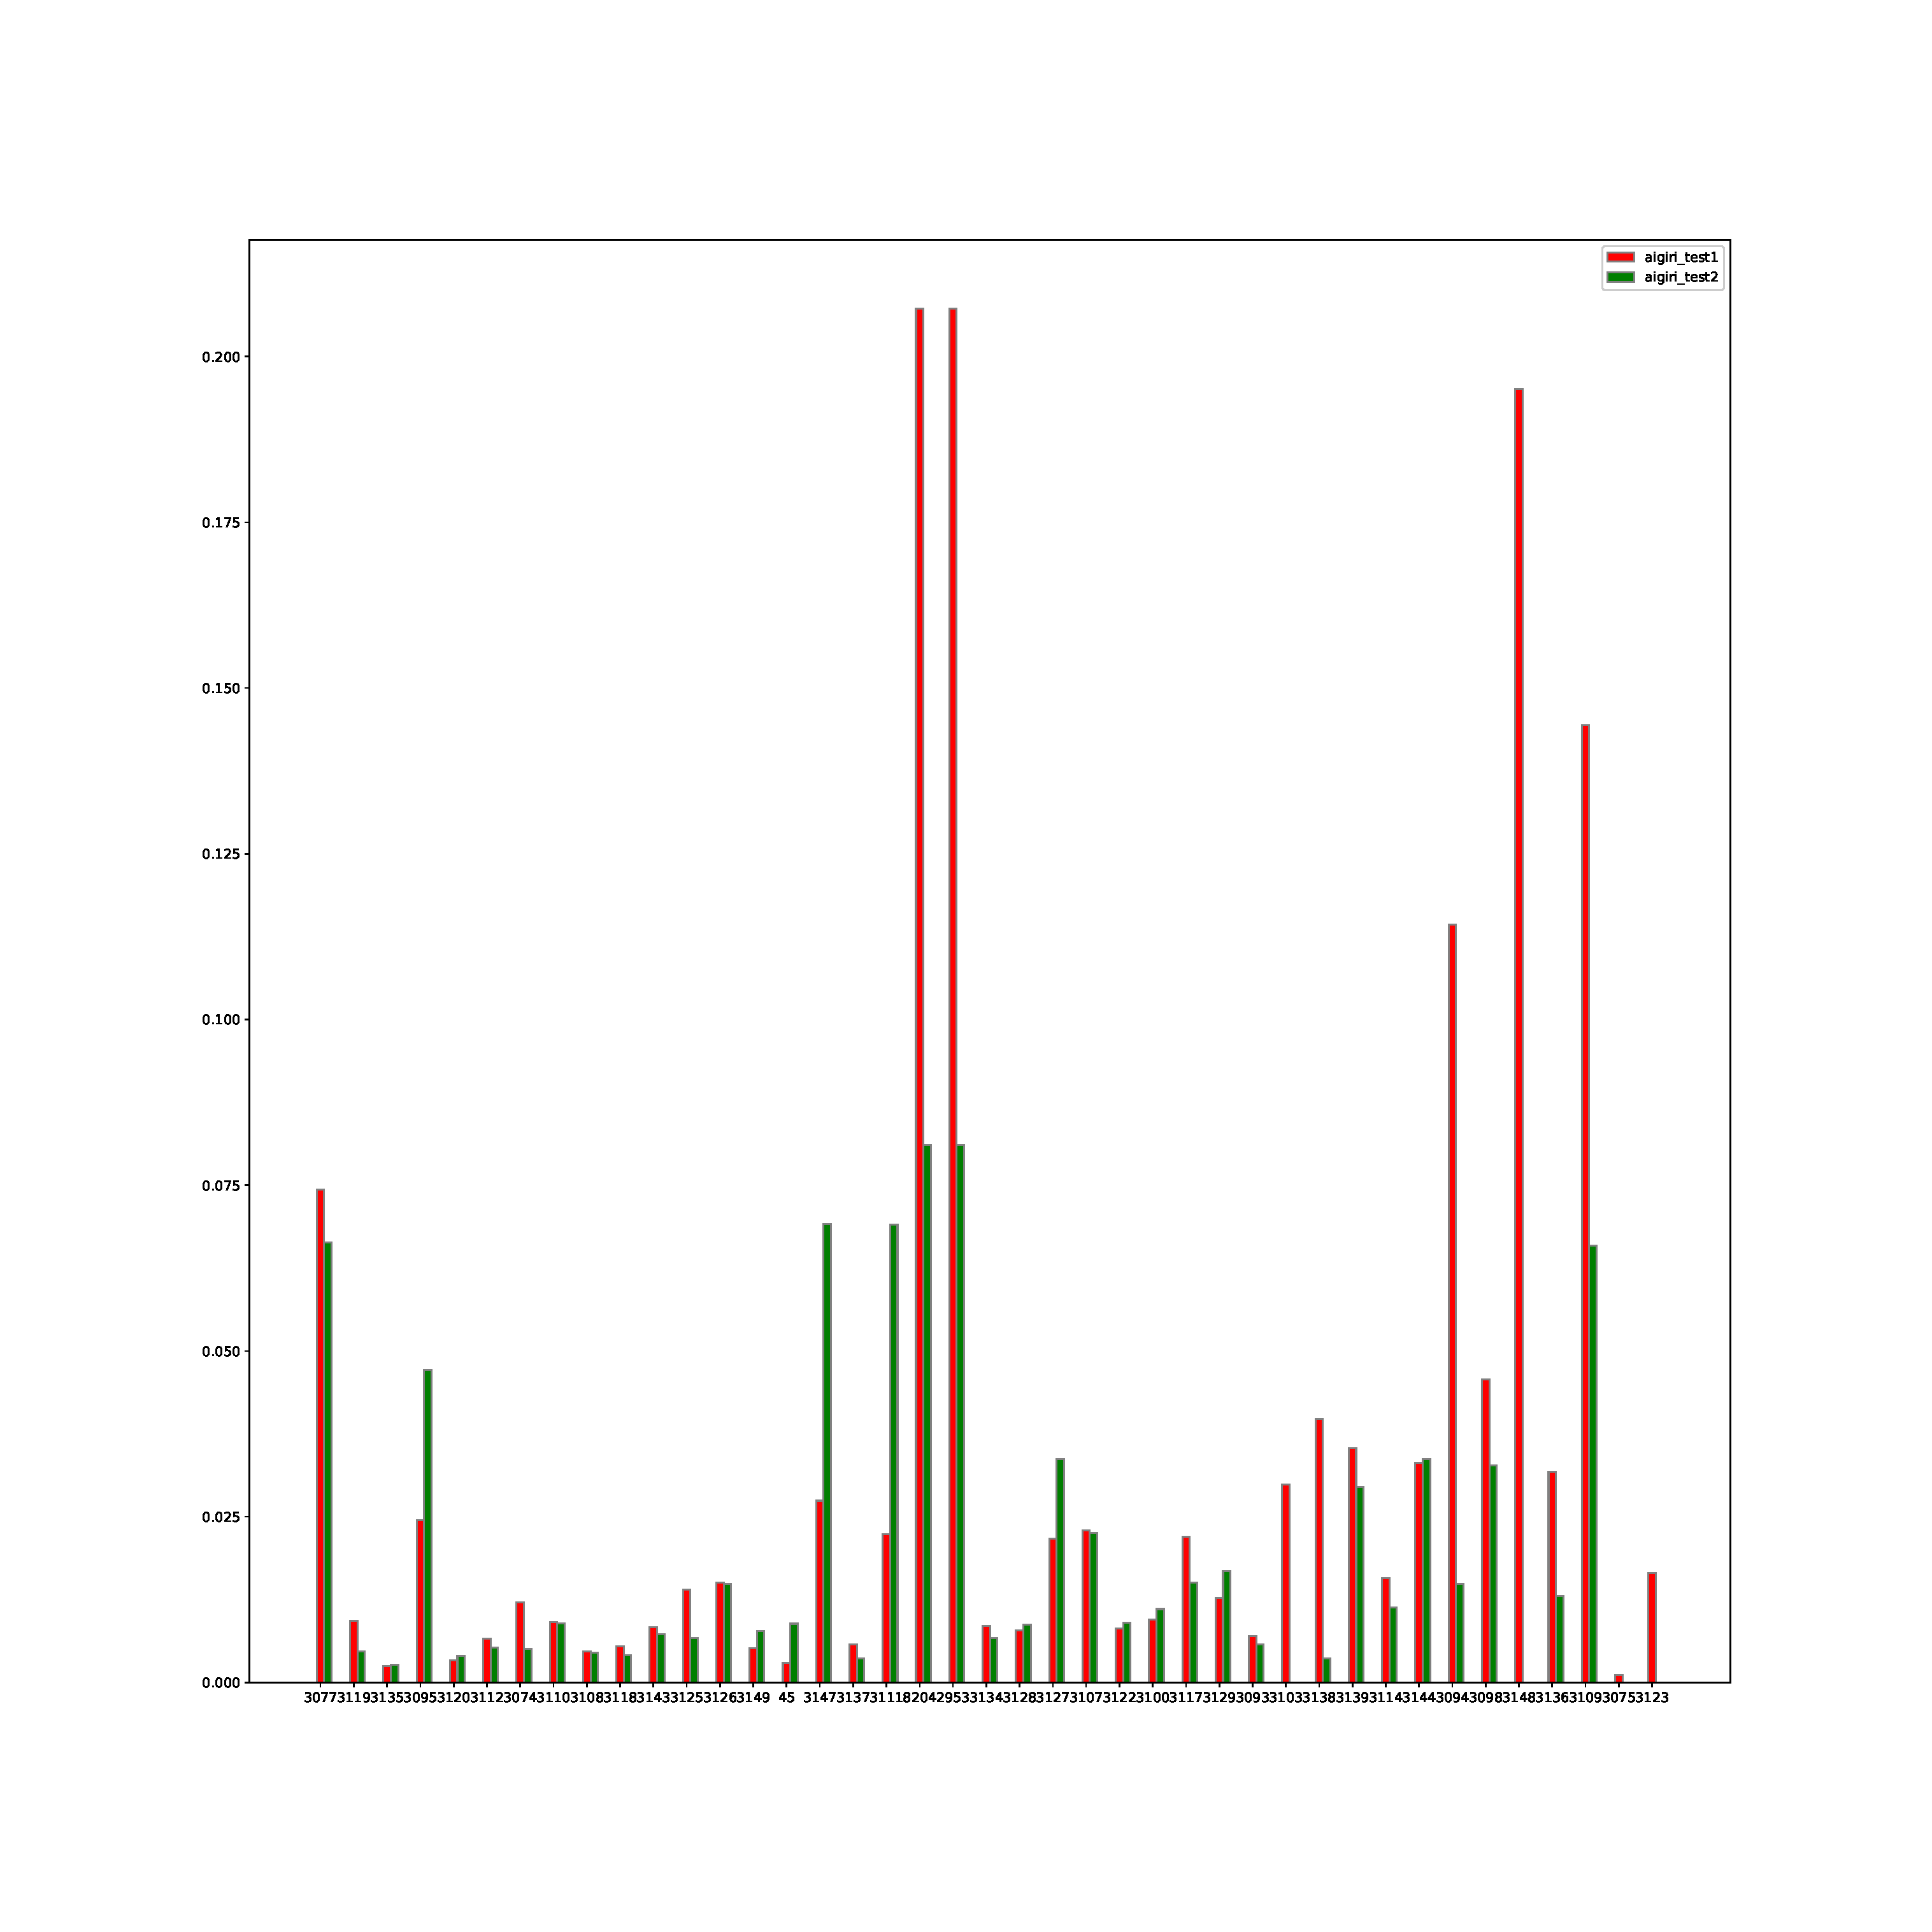
\includegraphics[width=\columnwidth]{./figs/normalized.eps}
\caption{Bar graph depicitng the periodicity of the common characters}
\label{fig:bar}
\end{figure} 

\end{enumerate}
